\section{Post-Exploitation}

\begin{figure}
  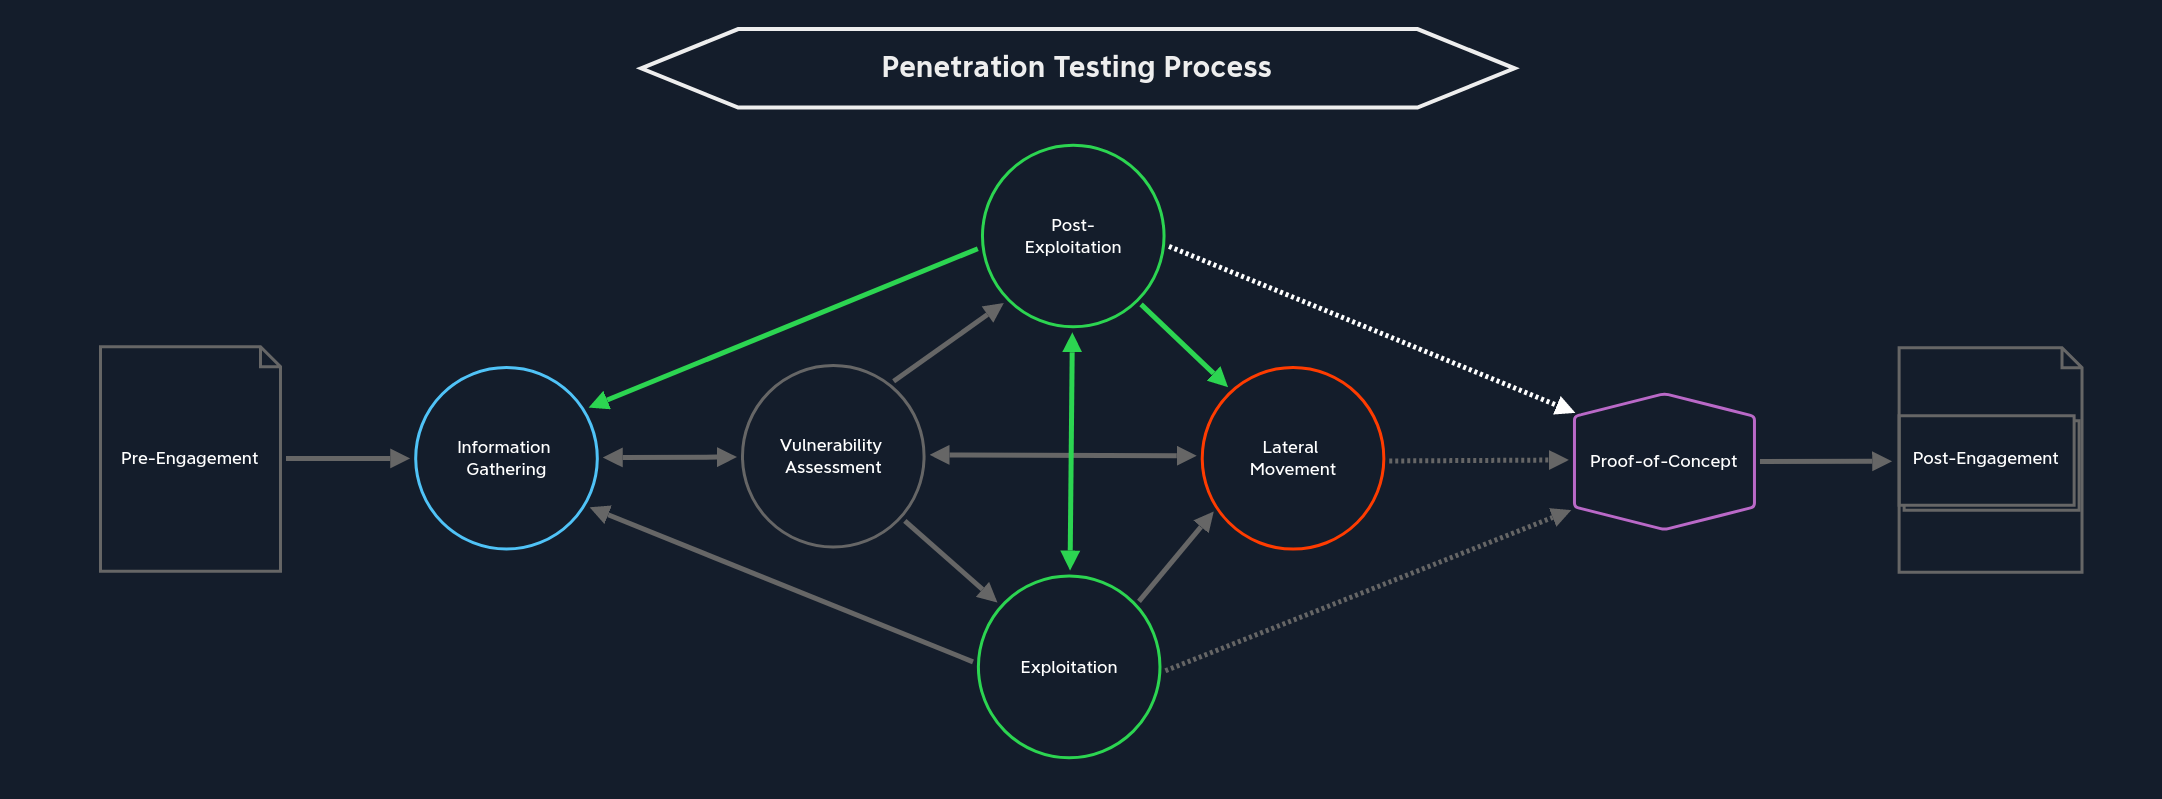
\includegraphics[width=\linewidth]{intro/process/images/post.png}
  \caption{Post-Exploitation}
  \label{fig:pentest-process-post-exploit}
\end{figure}

 The Post-Exploitation stage aims to obtain sensitive and security-relevant
 information from a local perspective and business-relevant information that,
 in most cases, requires higher privileges than a standard user. This stage
 includes the following components:

 \begin{tabular}{ll}
 Evasive Testing &	Information Gathering \\
Pillaging &	Vulnerability Assessment \\
Privilege Escalation &	Persistence \\
Data Exfiltration & \\
\end{tabular}

\subsection{Evasive Testing}
If a skilled administrator monitors the systems, any change or even a single
command could trigger an alarm that will give us away. In many cases, we get
kicked out of the network, and then threat hunting begins where we are the
focus. We may also lose access to a host (that gets quarantined) or a user
account (that gets temporarily disabled or the password changed). This
penetration test would have failed but succeeded in some ways because the
client could detect some actions. We can provide value to the client in this
situation by still writing up an entire attack chain and helping them identify
gaps in their monitoring and processes where they did not notice our actions.
For us, we can study how and why the client detected us and work on improving
our evasion skills. Perhaps we did not thoroughly test a payload, or we got
careless and ran a command such as \verb+net user+ or \verb+whoami+ that is
often monitored by EDR systems and flagged as anomalous activity. 

Evasive testing is divided into three different categories:
Evasive, Hybrid Evasive and Non-Evasive

This does not mean that we cannot use all three methods. Suppose our client
wants to perform an intrusive penetration test to get as much information as
possible and the most in-depth testing results. In that case, we will perform
Non-Evasive Testing, as the security measures around the network may limit and
even stop us. However, this can also be combined with Evasive testing, using
the same commands and methods for non-evasive testing. We can then see if the
security measures can identify and respond to the actions performed. In
Hybrid-Evasive testing, we can test specific components and security measures
that have been defined in advance. This is common when the customer only wants
to test specific departments or servers to see if they can withstand the
attacks.

\subsection{Information Gathering}

Since we have gained a new perspective on the system and the network of our
target system in the Exploitation stage, we are basically in a new environment.
This means we first have to reacquaint ourselves with what we are working with
and what options are available. Therefore, in the Post-Exploitation stage, we
go through the Information Gathering and Vulnerability Assessment stages again,
which we can consider as parts of the current stage. This is because the
information we had up to this point was gathered from an external perspective,
not an internal one.

From the inside (local) perspective, we have many more possibilities and
alternatives to access certain information that is relevant to us. Therefore,
the information gathering stage starts all over again from the local
perspective. We search and gather as much information as we can. The difference
here is that we also enumerate the local network and local services such as
printers, database servers, virtualization services, etc. Often we will find
shares intended for employees to use to exchange and share data and files. The
investigation of these services and network components is called Pillaging.

\subsection{Pillaging}

Pillaging is the stage where we examine the role of the host in the corporate
network. We analyze the network configurations, including but not limited to:
Interfaces, Routing, DNS, ARP\ldots

Understanding the role of the system we are on also gives us an excellent
understanding of how it communicates with other network devices and its
purpose. From this, we can find out, for example, what alternative subdomains
exist, whether it has multiple network interfaces, whether there are other
hosts with which this system communicates, if admins are connecting to other
hosts from it, and if we can potentially reuse credentials or steal an SSH key
to further our access or establish persistence, etc. This helps, above all, to
get an overview of the network's structure.

During the pillaging stage, we will also hunt for sensitive data such as
passwords on shares, local machines, in scripts, configuration files, password
vaults, documents (Excel, Word, .txt files, etc.), and even email.

Our main goals with pillaging are to show the impact of successful exploitation
and, if we have not yet reached the goal of the assessment, to find additional
data such as passwords that can be inputs to other stages such as lateral
movement. 


\subsection{Persistence}

Once we have an overview of the system, our immediate next step is maintaining
access to the exploited host. This way, if the connection is interrupted, we
can still access it. This step is essential and often used as the first step
before the Information Gathering and Pillaging stages.

We should follow non-standardized sequences because each system is individually
configured by a unique administrator who brings their own preferences and
knowledge. It is recommended that we work flexibly during this phase and adapt
to the circumstances. For example, suppose we have used a buffer overflow
attack on a service that is likely to crash it. In that case, we should
establish persistence to the system as soon as possible to avoid having to
attack the service multiple times and potentially causing a disruption. Often
if we lose the connection, we will not be able to access the system in the same
way.

\subsection{Vulnerability Assessment}

If we can maintain access and have a good overview of the system, we can use
the information about the system and its services and any other data stored on
it to repeat the Vulnerability Assessment stage, but this time from inside the
system. We analyze the information and prioritize it accordingly. The goal we
pursue next is the escalation of privileges (if not already in place).

Again, it is essential to distinguish between exploits that can harm the system
and attacks against the services that do not cause any disruption. In doing so,
we weigh the components we have already gone through in the first Vulnerability
Assessment stage.

\subsection{Privilege Escalation}

Privilege escalation is significant, and in most cases, it represents a
critical moment that can open many more new doors for us. Getting the highest
possible privileges on the system or domain is often crucial. Therefore we want
to get the privileges of the root (on Linux-based systems) or the domain
administrator/local administrator/SYSTEM (on Windows-based systems) because
this will often allow us to move through the entire network without any
restrictions.

However, it is essential to remember that the escalation of privileges does not
always have to occur locally on the system. We can also obtain stored
credentials during the information gathering stage from other users who are
members of a higher privileged group. Exploiting these privileges to log in as
another user is also part of privilege escalation because we have escalated our
privileges (quickly) using the new set of credentials.

\subsection{Data Exfiltration}

During the Information Gathering and Pillaging stage, we will often be able to
find, among other things, considerable personal information and customer data.
Some clients will want to check whether it is possible to exfiltrate these
types of data. Security systems such as Data Loss Prevention (DLP) and
Endpoint Detection and Response (EDR) help detect and prevent data
exfiltration. In addition to Network Monitoring, many companies use encryption
on hard drives to prevent external parties from viewing such information.
Before exfiltrating any actual data, we should check with the customer and our
manager. It can often be enough to create some bogus data (such as fake credit
card numbers or social security numbers) and exfiltrate it to our system. That
way, the protection mechanisms that look for patterns in data leaving the
network will be tested, but we will not be responsible for any live sensitive
data on our testing machine.

Companies must adhere to data security regulations depending on the type of
data involved. These include, but are not limited to:
Credit Card Account Information (Payment Card Industry (PCI)), Electronic
Patient Health Information 'Health Insurance Portability and Accountability Act
(HIPAA)), Consumers Private Banking Information (Gramm-Leach-Bliley (GLBA))
Government Information 	(Federal Information Security Management Act of 2002
(FISMA))

It is worth familiarizing ourselves with each of these frameworks but what is
crucial for us, however, is how we handle this information. For us, the type of
data does not have much significance, but the required controls around it do,
and as stated previously, we can simulate exfiltrating data from the network as
a proof of concept that it is possible. We should check with the client to
ensure that their systems are intended to catch the fake data type that we
attempt to exfiltrate if we are successful, so we do not misrepresent anything
in our report.

It's a good habit to run a screen recording (along with taking screenshots) as
additional evidence for such vital steps. If we only have terminal access, we
can display the hostname, IP address, user name, and the corresponding path to
the customer file and take a screenshot or screen capture. This helps us prove
where the data originated from and that we could remove it from the environment
successfully.

If sensitive data like this is found, our client should, of course, be informed
immediately. Based on the fact that we could escalate the privileges and
exfiltrate personal data, they may want to pause, end, or shift the focus of
the penetration test, especially if data exfiltration was the primary goal.
However, this is at our client's discretion, and many will prefer that we keep
testing to identify all possible weaknesses in their environment.

